\chapter{Équilibres d'oxydoréduction et relation de Nernst}\label{ch:b1:nernst}

Plaçons une lame de zinc dans une solution de sulfate de zinc, une lame
de cuivre dans une solution de sulfate de cuivre(II), relions les deux
solutions par un tube de solution saline et les deux métaux par un fil
passant par une diode électroluminescente~: la diode s'allume. La
réaction du zinc avec les ions cuivre, qui dans un seul bécher ne fait
que chauffer la solution, fait maintenant circuler des électrons dans un
fil. Une pile est ce montage, conditionné~; un pH-mètre et une électrode
à chlorure en sont les cousins de mesure. Ce chapitre rend quantitatif
l'échange d'électrons~: les \omterm{def:b1:nernst:oxidation-number}{nombres d'oxydation} pour compter les
électrons, les \omterm{def:b1:nernst:electrode-potential}{potentiels d'électrode} pour classer les couples, et la
\omterm{thm:b1:nernst:nernst}{relation de Nernst} pour suivre leur variation avec la concentration.

\begin{recall}
Le volume scolaire (années 11 et 12) a défini les \omterm{def:b1:nernst:couple}{oxydants} et les
\omterm{def:b1:nernst:couple}{réducteurs}, écrit des \omterm{def:b1:nernst:couple}{demi-équations}, construit des piles à partir de
deux métaux et de deux solutions, et présenté la pile zinc--cuivre comme
une batterie. Le \omterm{def:b1:extent-q-and-k:quotient}{quotient de réaction} et la constante d'équilibre sont
ceux du \cref{ch:b1:extent-q-and-k}~; les \omterm{def:b1:extent-q-and-k:activity}{activités} valent $c/c^\circ$
pour les solutés et $p/p^\circ$ pour les gaz, 1 pour les solides et les
liquides purs.
\end{recall}

\section{Nombres d'oxydation et couples}

\begin{definition}[Oxydant, réducteur, couple oxydant/réducteur, demi-équation]\label{def:b1:nernst:couple}
Un \emph{oxydant}\index{oxydant} est une espèce capable de capter des
électrons, un \emph{réducteur}\index{reducteur@réducteur} une espèce capable d'en céder. Un
oxydant Ox et le réducteur Red qu'il devient forment un \emph{couple
oxydant/réducteur}\index{couple oxydant/reducteur@couple oxydant/réducteur} Ox/Red, décrit par sa
\emph{demi-équation}\index{demi-equation@demi-équation}
$\alpha\,\mathrm{Ox} + n\,\mathrm{e^-} \rightleftharpoons
\beta\,\mathrm{Red}$, ajustée en atomes à l'aide de \ce{H2O} et de
\ce{H+} si nécessaire, et en charge à l'aide des électrons.
\end{definition}

Une réaction d'oxydoréduction est un échange d'électrons entre deux
couples~: l'\omterm{def:b1:nernst:couple}{oxydant} de l'un est réduit tandis que le \omterm{def:b1:nernst:couple}{réducteur} de
l'autre est oxydé, et les électrons se compensent. Pour les compter dans
une espèce compliquée, on attribue à chaque atome un \omterm{def:b1:nernst:oxidation-number}{nombre d'oxydation}.

\begin{definition}[Nombre d'oxydation]\label{def:b1:nernst:oxidation-number}
Le \emph{nombre d'oxydation}\index{nombre d'oxydation} d'un atome dans une
espèce est la charge qu'il porterait si chaque liaison était rompue en
donnant les deux électrons liants à l'atome le plus électronégatif
(partagés également entre deux atomes identiques). On l'écrit en chiffres
romains~: fer(III), \ce{Mn^{+VII}} dans l'ion permanganate.
\end{definition}

\begin{proposition}[Règles des nombres d'oxydation]\label{prop:b1:nernst:on-rules}
\begin{enumerate}
  \item Un atome dans un corps simple a le \omterm{def:b1:nernst:oxidation-number}{nombre d'oxydation} 0~; un ion
        monoatomique a pour \omterm{def:b1:nernst:oxidation-number}{nombre d'oxydation} sa charge.
  \item La somme des \omterm{def:b1:nernst:oxidation-number}{nombres d'oxydation} des atomes d'une espèce est
        égale à sa charge.
  \item L'hydrogène est à $+$I (sauf dans les hydrures métalliques,
        $-$I)~; l'oxygène est à $-$II (sauf dans les peroxydes, $-$I, et
        lié au fluor)~; le fluor est à $-$I.
  \item Dans une \omterm{def:b1:nernst:couple}{demi-équation}, le nombre d'électrons est égal à la
        variation du \omterm{def:b1:nernst:oxidation-number}{nombre d'oxydation} de l'élément qui change, multipliée
        par le nombre de ses atomes.
\end{enumerate}
\end{proposition}

\begin{proof}
1 et 2~: rompre toutes les liaisons conserve la charge, et entre atomes
identiques rien n'est transféré. 3~: l'hydrogène est moins
électronégatif que tous les non-métaux auxquels il se lie
(\cref{ch:b1:periodicity}) et plus que les métaux alcalins~; l'oxygène
est plus électronégatif que tous les éléments sauf le fluor, et dans
\ce{O-O} le doublet partagé est réparti également. 4~: H et O gardent
leurs nombres, de sorte que les seuls atomes dont la charge fictive
change sont ceux de l'élément concerné, et les électrons apparaissent
dans la \omterm{def:b1:nernst:couple}{demi-équation} exactement pour compenser cette variation de
charge.
\end{proof}

\begin{method}[Nombres d'oxydation d'une espèce]\label{met:b1:nernst:oxidation-numbers}
Donner à H, O, F et aux ions leurs nombres usuels~; celui de l'atome
restant découle de la règle 2. Dans \ce{MnO4-}~: $x + 4(-2) = -1$,
$x = +7$. Dans \ce{Cr2O7^2-}~: $2x - 14 = -2$, $x = +6$. Dans
\ce{S4O6^2-}, la moyenne vaut
$+2.5$~; le \omterm{def:b1:lewis-resonance-vsepr:lewis}{schéma de Lewis} montre deux sortes de soufre.
\end{method}

\begin{method}[Ajuster une demi-équation]\label{met:b1:nernst:balance-by-on}
\begin{enumerate}
  \item Ajuster l'élément dont le \omterm{def:b1:nernst:oxidation-number}{nombre d'oxydation} change.
  \item Ajouter les électrons~: la variation du \omterm{def:b1:nernst:oxidation-number}{nombre d'oxydation}
        multipliée par le nombre d'atomes.
  \item Ajuster la charge avec \ce{H+} (solution acide) ou \ce{OH-}
        (solution basique).
  \item Ajuster l'hydrogène et l'oxygène avec \ce{H2O}~; vérifier
        l'oxygène en dernier.
\end{enumerate}
Pour l'ion permanganate en milieu acide~: Mn passe de $+$VII à $+$II,
donc 5 électrons~; la charge vaut $-1 - 5 = -6$ à gauche et $+2$ à
droite, d'où $8\,\ce{H+}$~; puis $4\,\ce{H2O}$~:
\ce{MnO4- + 8H+ + 5e- -> Mn^2+ + 4H2O}.
\end{method}

\section{Piles électrochimiques}

\begin{definition}[Pile électrochimique]\label{def:b1:nernst:cell}
Une \emph{pile électrochimique}\index{pile electrochimique@pile électrochimique} est formée de deux
\emph{demi-piles}\index{demi-pile}, chacune constituée d'un couple et
d'un conducteur électronique, l'électrode, reliées par un conducteur
ionique, souvent un \emph{pont salin}\index{pont salin} (un gel ou un
tube contenant un sel inerte concentré comme le nitrate de potassium).
L'électrode où a lieu l'oxydation est l'\emph{anode}\index{anode}, celle
où a lieu la réduction la \emph{cathode}\index{cathode}. La
\emph{tension à vide}\index{tension a vide@tension à vide} de la pile est la différence de potentiel
électrique entre les deux électrodes, pôle positif moins pôle négatif,
mesurée lorsqu'aucun courant ne circule.
\end{definition}

\begin{omfigure}
\begin{tikzpicture}[font=\small, >={Stealth}]
  \pic at (0,0) {beaker={0.7}{omDef!14}};
  \pic at (3.6,0) {beaker={0.7}{omDef!32}};
  \pic at (-0.3,0.25) {electrode={black!35}};
  \pic at (3.9,0.25) {electrode={orange!70!brown}};
  \pic at (0.35,0.55) {saltbridge={2.9}};
  \pic (m) at (1.8,4.3) {meter={V}};
  \draw[thick] (-0.15,2.65) |- (m-a);
  \draw[thick] (4.05,2.65) |- (m-b);
  \node[anchor=east] at (-0.95,1.0) {\ce{Zn}};
  \node[anchor=west] at (4.45,1.0) {\ce{Cu}};
  \node at (0.25,-0.35) {\ce{Zn^2+}, \ce{SO4^2-}};
  \node at (3.6,-0.35) {\ce{Cu^2+}, \ce{SO4^2-}};
  \draw[->, omProp, thick] (-0.15,3.35) -- (0.8,3.35) node[above, midway] {$\mathrm{e^-}$};
  \draw[->, omProp, thick] (2.8,3.35) -- (3.75,3.35) node[above, midway] {$\mathrm{e^-}$};
  \node[anchor=east] at (-0.9,2.3) {$-$ anode};
  \node[anchor=west] at (4.6,2.3) {cathode $+$};
  \node[font=\scriptsize, align=center] at (1.8,2.75) {pont salin\\ \ce{K+} $\rightarrow$ \quad $\leftarrow$ \ce{NO3-}};
  \node[font=\scriptsize] at (-0.1,-0.8) {\ce{Zn -> Zn^2+ + 2e-}};
  \node[font=\scriptsize] at (3.7,-0.8) {\ce{Cu^2+ + 2e- -> Cu}};
\end{tikzpicture}

{\small La pile zinc--cuivre (pile Daniell). Le zinc est oxydé à
l'\omterm{def:b1:nernst:cell}{anode}, le pôle négatif~; les ions cuivre sont réduits à la \omterm{def:b1:nernst:cell}{cathode}, le
pôle positif. Les électrons circulent dans le circuit extérieur du zinc
vers le cuivre~; dans le \omterm{def:b1:nernst:cell}{pont salin}, les cations se déplacent vers la
\omterm{def:b1:nernst:cell}{cathode} et les anions vers l'\omterm{def:b1:nernst:cell}{anode}, ce qui maintient chaque solution
neutre.}
\end{omfigure}

Une pile s'écrit sur une ligne, l'\omterm{def:b1:nernst:cell}{anode} à gauche~: \ce{Zn} $|$ \ce{Zn^2+}
$\|$ \ce{Cu^2+} $|$ \ce{Cu}, un trait simple pour les interfaces, un
double trait pour le \omterm{def:b1:nernst:cell}{pont salin}. Toutes les concentrations étant à
\qty{1}{mol/L}, sa tension vaut \qty{1.10}{V}. La réaction qui a lieu
quand la pile débite, \ce{Zn + Cu^2+ -> Zn^2+ + Cu}, est celle qui se
produirait dans un seul bécher~; séparer les \omterm{def:b1:nernst:cell}{demi-piles} oblige les
électrons à passer par le fil, où ils peuvent fournir un travail.

\section{Potentiels d'électrode}

Une tension est une différence~: on ne peut mesurer que des différences
entre deux \omterm{def:b1:nernst:cell}{demi-piles}. On choisit donc une fois pour toutes une
\omterm{def:b1:nernst:cell}{demi-pile} de référence.

\begin{definition}[Potentiel d'électrode, potentiel standard]\label{def:b1:nernst:electrode-potential}
L'\emph{électrode standard à hydrogène}\index{electrode standard a hydrogene@électrode standard à hydrogène}
est une électrode de platine au contact de dihydrogène gazeux sous
\qty{1}{bar} et d'une solution idéale de \ce{H+} d'\omterm{def:b1:extent-q-and-k:activity}{activité} 1. Le
\emph{potentiel d'électrode}\index{potentiel d'electrode@potentiel d'électrode} $E$ d'une \omterm{def:b1:nernst:cell}{demi-pile} est la
tension de la pile qu'elle forme avec l'électrode standard à hydrogène
placée à gauche~:
$E = V_{\text{demi-pile}} - V_{\text{ESH}}$. Lorsque toutes les espèces du
couple ont une \omterm{def:b1:extent-q-and-k:activity}{activité} égale à 1, c'est le \emph{potentiel standard}\index{potentiel standard}
$E^\circ$ du couple, constante à une température donnée.
\end{definition}

\begin{omfigure}
\begin{tikzpicture}[font=\small, >={Stealth}]
  \pic at (0,0) {beaker={0.72}{omDef!14}};
  % glass jacket, open at the bottom, with the gas inlet on the right
  \draw[om glass] (-0.32,0.35) -- (-0.32,3.0) -- (0.32,3.0) -- (0.32,2.55)
    -- (0.95,2.55) (0.32,2.35) -- (0.95,2.35) (0.32,2.35) -- (0.32,0.35);
  \draw[thick] (0,0.9) -- (0,3.45);
  \fill[black!60] (-0.16,0.5) rectangle (0.16,0.9);
  \foreach \x/\y in {0.45/0.45, 0.55/0.75, 0.48/1.05, -0.45/0.5, -0.52/0.85}
    \draw[omDef!70] (\x,\y) circle (0.055);
  \draw[->] (1.9,2.45) node[right] {\ce{H2}, \qty{1}{bar}} -- (1.0,2.45);
  \draw (0.12,0.7) -- (1.5,0.2) node[right] {platine platiné};
  \draw (-0.6,1.1) -- (-1.4,1.6) node[left] {\ce{H+}, activité 1};
  \node[anchor=west] at (0.05,3.45) {vers le circuit};
\end{tikzpicture}

{\small L'\omterm{def:b1:nernst:electrode-potential}{électrode standard à hydrogène}~: du dihydrogène gazeux barbote
sur une plaque de platine recouverte de platine finement divisé, plongée
dans une solution où \ce{H+} a une \omterm{def:b1:extent-q-and-k:activity}{activité} égale à 1. Son couple est
\ce{H+}/\ce{H2}, de potentiel nul par convention.}
\end{omfigure}

L'électrode à hydrogène est malcommode~; les laboratoires mesurent par
rapport à une \omterm{def:b1:nernst:cell}{demi-pile} plus pratique, dont le potentiel est connu.

\begin{definition}[Électrode de référence]\label{def:b1:nernst:reference-electrode}
Une \emph{électrode de référence}\index{electrode de reference@électrode de référence} est une \omterm{def:b1:nernst:cell}{demi-pile}
dont le potentiel est fixé et connu~: l'électrode argent--chlorure
d'argent (un fil d'argent recouvert de chlorure d'argent dans une
solution de chlorure de concentration fixée) ou l'électrode au calomel
(du mercure au contact de \ce{Hg2Cl2} et d'une solution de chlorure).
\end{definition}

Le tableau ci-dessous donne les \omterm{def:b1:nernst:electrode-potential}{potentiels standard} utilisés dans ce
volume~; l'échelle verticale de la section suivante montre les plus
courants.

\begin{omfigure}
\begin{tabular}{lr@{\qquad}lr}
\hline
couple & $E^\circ$ (V) & couple & $E^\circ$ (V) \\
\hline
\ce{Li+}/\ce{Li} & $-3.04$ & \ce{Cu^2+}/\ce{Cu} & 0.34 \\
\ce{K+}/\ce{K} & $-2.94$ & $[\ce{Fe(CN)6}]^{3-}$/$[\ce{Fe(CN)6}]^{4-}$ & 0.36 \\
\ce{Na+}/\ce{Na} & $-2.71$ & \ce{Cu+}/\ce{Cu} & 0.52 \\
\ce{Mg^2+}/\ce{Mg} & $-2.36$ & \ce{I2}/\ce{I-} & 0.53 \\
\ce{Al^3+}/\ce{Al} & $-1.68$ & \ce{O2}/\ce{H2O2} & 0.69 \\
\ce{Zn^2+}/\ce{Zn} & $-0.76$ & \ce{Fe^3+}/\ce{Fe^2+} & 0.77 \\
\ce{Fe^2+}/\ce{Fe} & $-0.41$ & \ce{Hg2^2+}/\ce{Hg} & 0.80 \\
\ce{Ni^2+}/\ce{Ni} & $-0.24$ & \ce{Ag+}/\ce{Ag} & 0.80 \\
\ce{Pb^2+}/\ce{Pb} & $-0.13$ & \ce{Br2}/\ce{Br-} & 1.08 \\
\ce{H+}/\ce{H2} & 0 & \ce{O2}/\ce{H2O} & 1.23 \\
\ce{S4O6^2-}/\ce{S2O3^2-} & 0.02 & \ce{MnO2}/\ce{Mn^2+} & 1.23 \\
\ce{Cu^2+}/\ce{Cu+} & 0.16 & \ce{Cl2}/\ce{Cl-} & 1.36 \\
\ce{AgCl}/\ce{Ag} & 0.22 & \ce{PbO2}/\ce{Pb^2+} & 1.46 \\
\ce{Hg2Cl2}/\ce{Hg} & 0.27 & \ce{MnO4-}/\ce{Mn^2+} & 1.51 \\
 & & \ce{HClO}/\ce{Cl2} & 1.63 \\
 & & \ce{H2O2}/\ce{H2O} & 1.76 \\
\hline
\end{tabular}

\smallskip
{\small \omterm{def:b1:nernst:electrode-potential}{Potentiels standard} à \qty{25}{\celsius}, calculés à partir des
enthalpies libres standard de formation tabulées des espèces de chaque
couple. Ils peuvent différer de quelques centièmes de volt d'autres
compilations.}
% ledger: dfg:Li+_ao, dfg:K+_ao, dfg:Na+_ao, dfg:Mg2+_ao, dfg:Al3+_ao, dfg:Zn2+_ao, dfg:Fe2+_ao, dfg:Ni2+_ao, dfg:Pb2+_ao (computed in figdata/bachelor-1/standard-potentials.py)
% ledger: dfg:S4O62-_ao, dfg:S2O32-_ao, dfg:Cu2+_ao, dfg:Cu+_ao, dfg:AgCl_cr, dfg:Cl-_ao, dfg:Hg2Cl2_cr, dfg:Fe_CN63-_ao, dfg:Fe_CN64-_ao, dfg:I-_ao (same script)
% ledger: dfg:H2O2_ao, dfg:Fe3+_ao, dfg:Hg22+_ao, dfg:Ag+_ao, dfg:Br-_ao, dfg:H2O_l, dfg:MnO2_cr, dfg:Mn2+_ao, dfg:PbO2_cr, dfg:MnO4-_ao, dfg:HClO_ao (same script)
\end{omfigure}

\section{La relation de Nernst}

\begin{theorem}[Relation de Nernst]\label{thm:b1:nernst:nernst}
Pour un couple $\alpha\,\mathrm{Ox} + n\,\mathrm{e^-} \rightleftharpoons
\beta\,\mathrm{Red}$, avec éventuellement d'autres espèces (\ce{H+},
\ce{H2O}, \ce{Cl-}) d'un côté ou de l'autre, le \omterm{def:b1:nernst:electrode-potential}{potentiel d'électrode} est
donné par la \emph{relation de Nernst}\index{relation de Nernst}
\[
  E = E^\circ + \frac{RT}{nF}\ln\frac{\prod a_{\text{côté ox}}^{\nu}}{\prod
  a_{\text{côté red}}^{\nu}}
  = E^\circ + \frac{0.059}{n}\log\frac{a(\mathrm{Ox})^\alpha\,\cdots}{a(\mathrm{Red})^\beta\,\cdots}
  \quad\text{à \qty{25}{\celsius}},
\]
où chaque \omterm{def:b1:extent-q-and-k:activity}{activité} porte son \omterm{def:b1:extent-q-and-k:extent}{nombre stœchiométrique}, le facteur valant
$RT\ln 10/F = \qty{0.059}{V}$ à \qty{298}{K}.
\end{theorem}

\admitted{La \omterm{thm:b1:nernst:nernst}{relation de Nernst} découle du lien entre l'enthalpie libre
d'une réaction et la tension de la pile, établi dans le volume de
deuxième année.}

\begin{example}[Trois couples]\label{ex:b1:nernst:examples}
\ce{Cu^2+}/\ce{Cu}~: $E = 0.34 + 0.030\log[\ce{Cu^2+}]$ (le cuivre
métallique a une \omterm{def:b1:extent-q-and-k:activity}{activité} égale à 1).
\ce{Fe^3+}/\ce{Fe^2+}~: $E = 0.77 + 0.059\log([\ce{Fe^3+}]/[\ce{Fe^2+}])$.
\ce{MnO4-}/\ce{Mn^2+}~: $E = 1.51 + \frac{0.059}{5}\log
\frac{[\ce{MnO4-}][\ce{H+}]^8}{[\ce{Mn^2+}]}$~; à concentrations égales
en permanganate et en manganèse(II), $E = 1.51 - 0.094\,\mathrm{pH}$~: le
pouvoir \omterm{def:b1:nernst:couple}{oxydant} du permanganate diminue quand le pH augmente.
\end{example}

Une variation d'un facteur dix d'une concentration déplace le potentiel
de $0.059/n$ volt~: quelques dizaines de millivolts. C'est pourquoi une
tension mesurée au millivolt près est une mesure précise d'une
concentration~: c'est le principe de l'électrode de verre du pH-mètre et
de l'électrode à chlorure du problème du week-end.

\begin{history}[Walther Nernst]
\begin{minipage}[t]{0.22\linewidth}\vspace{0pt}
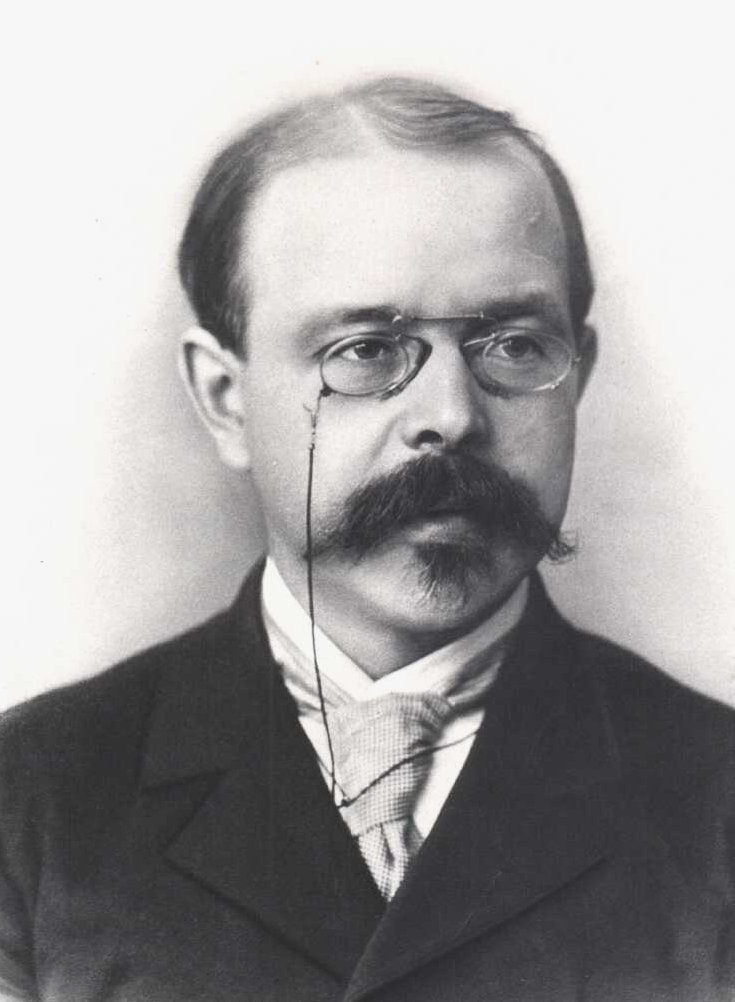
\includegraphics[width=\linewidth]{images/book2/nernst.jpg}
\end{minipage}\hfill
\begin{minipage}[t]{0.74\linewidth}\vspace{0pt}
Walther Nernst (1864--1941), ici à vingt-cinq ans, en 1889. La relation
de cette section, qui relie la tension d'une pile aux concentrations de
ses ions, porte son nom, de même qu'un troisième principe de la
thermodynamique rencontré dans le volume de deuxième année.
(Photographie~: Smithsonian Libraries, domaine public, Wikimedia
Commons.)
\end{minipage}
\end{history}

\section{Prévoir les réactions d'oxydoréduction}

\begin{method}[Prévoir une réaction d'oxydoréduction]\label{met:b1:nernst:predict-redox}
\begin{enumerate}
  \item Placer les couples sur une échelle verticale de \omterm{def:b1:nernst:electrode-potential}{potentiels
        standard}, les \omterm{def:b1:nernst:couple}{oxydants} à gauche, les \omterm{def:b1:nernst:couple}{réducteurs} à droite.
  \item L'\omterm{def:b1:nernst:couple}{oxydant} le plus fort présent (le plus grand $E^\circ$) réagit
        avec le \omterm{def:b1:nernst:couple}{réducteur} le plus fort présent (le plus petit
        $E^\circ$)~: la flèche qui descend de l'\omterm{def:b1:nernst:couple}{oxydant} au \omterm{def:b1:nernst:couple}{réducteur},
        puis remonte vers les produits, dessine un gamma grec, $\gamma$.
  \item La réaction est favorable ($K > 1$) lorsque le couple de
        l'\omterm{def:b1:nernst:couple}{oxydant} est au-dessus de celui du \omterm{def:b1:nernst:couple}{réducteur}~; elle est
        \omterm{def:b1:extent-q-and-k:quantitative}{quantitative} en pratique lorsque l'écart dépasse \qty{0.25}{V}
        environ pour un électron échangé.
\end{enumerate}
\end{method}

\begin{omfigure}
\begin{tikzpicture}[font=\small, >={Stealth}, y=2.6cm]
  \draw[->, thick] (0,-1.0) -- (0,1.85) node[above] {$E^\circ$ (V)};
  \foreach \e/\o/\r in {-0.76/\ce{Zn^2+}/\ce{Zn}, 0/\ce{H+}/\ce{H2},
      0.34/\ce{Cu^2+}/\ce{Cu}, 0.77/\ce{Fe^3+}/\ce{Fe^2+},
      1.36/\ce{Cl2}/\ce{Cl-}, 1.51/\ce{MnO4-}/\ce{Mn^2+}} {
    \draw (-0.12,\e) -- (0.12,\e);
    \node[anchor=east] at (-0.25,\e) {\o};
    \node[anchor=west] at (0.25,\e) {\r};
    \node[anchor=west, black!55, font=\scriptsize] at (2.0,\e) {\e};
  }
  \node[omProp] at (-1.0,1.85) {oxydants};
  \node[omDef] at (1.1,1.85) {réducteurs};
  % the gamma: Cu2+ meets Zn below it on the other side
  \draw[omThm, very thick, ->, rounded corners=4pt] (-1.0,0.28) -- (-1.0,-0.42) -- (0.6,-0.70);
  \draw[omThm, thick, ->] (-0.5,0.40) to[bend left=40] (0.5,0.40);
  \draw[omThm, thick, ->] (0.5,-0.85) to[bend left=40] (-0.5,-0.85);
\end{tikzpicture}

{\small Une échelle de \omterm{def:b1:nernst:electrode-potential}{potentiels standard}. La règle du gamma~:
l'\omterm{def:b1:nernst:couple}{oxydant} \ce{Cu^2+} réagit avec le \omterm{def:b1:nernst:couple}{réducteur} \ce{Zn}, situé plus bas de
l'autre côté (flèche épaisse)~; \ce{Cu^2+} est réduit en \ce{Cu} (flèche
courbe du haut) et \ce{Zn} oxydé en \ce{Zn^2+} (flèche courbe du bas).
La réaction inverse, \ce{Cu} avec \ce{Zn^2+}, n'est pas favorable.}
\end{omfigure}

\begin{proposition}[Constante d'équilibre et potentiels standard]\label{prop:b1:nernst:equilibrium-constant}
Pour la réaction $\mathrm{Ox_1} + \mathrm{Red_2} \rightleftharpoons
\mathrm{Red_1} + \mathrm{Ox_2}$ qui échange $n$ électrons,
\[
  \log K = \frac{n\,(E^\circ_1 - E^\circ_2)}{0.059}\quad\text{à \qty{25}{\celsius}} .
\]
\end{proposition}

\begin{proof}
À l'équilibre, aucun courant ne circule dans une pile construite à partir
des deux couples~: les deux électrodes ont le même potentiel, $E_1 = E_2$.
On écrit la \omterm{thm:b1:nernst:nernst}{relation de Nernst} de chacun avec le même $n$~:
$E^\circ_1 + \frac{0.059}{n}\log
\frac{a(\mathrm{Ox_1})}{a(\mathrm{Red_1})} = E^\circ_2 + \frac{0.059}{n}\log
\frac{a(\mathrm{Ox_2})}{a(\mathrm{Red_2})}$, donc $\frac{n(E^\circ_1 -
E^\circ_2)}{0.059} = \log\frac{a(\mathrm{Red_1})a(\mathrm{Ox_2})}{a(\mathrm{Ox_1})
a(\mathrm{Red_2})} = \log K$, les \omterm{def:b1:extent-q-and-k:activity}{activités} étant celles de l'équilibre.
\end{proof}

Pour la réaction de la pile Daniell, $\log K = 2(0.34 + 0.76)/0.059 = 37$~:
le zinc réduit totalement les ions cuivre. Pour
\ce{2Fe^3+ + 2I- <=> 2Fe^2+ + I2},
$\log K = 2(0.77 - 0.53)/0.059 = 8.1$. Le critère de la méthode en
découle~: avec $n = 1$, un écart de \qty{0.25}{V} donne $K = 10^{4.2}$.

\begin{proposition}[Combinaison de potentiels]\label{prop:b1:nernst:combined-potentials}
Si les couples $\mathrm{A}/\mathrm{B}$ ($n_1$ électrons) et
$\mathrm{B}/\mathrm{C}$ ($n_2$) se combinent en $\mathrm{A}/\mathrm{C}$
($n_3 = n_1 + n_2$), alors $n_3 E^\circ_3 = n_1 E^\circ_1 + n_2 E^\circ_2$.
Les potentiels ne s'additionnent pas~; les potentiels pondérés par les
électrons, si.
\end{proposition}

\begin{proof}
Dans une solution contenant A, B et C en équilibre avec une même
électrode, les trois couples ont le même potentiel $E$. On multiplie la
\omterm{thm:b1:nernst:nernst}{relation de Nernst} du premier par $n_1$, celle du second par $n_2$, et
on les additionne~: l'\omterm{def:b1:extent-q-and-k:activity}{activité} de B s'élimine et
$(n_1 + n_2)E = n_1E^\circ_1 + n_2E^\circ_2 +
0.059\log\frac{a(\mathrm{A})}{a(\mathrm{C})}$, ce qui est $n_3$ fois la
\omterm{thm:b1:nernst:nernst}{relation de Nernst} de A/C avec le $E^\circ_3$ annoncé.
\end{proof}

Cuivre~: $2E^\circ(\ce{Cu^2+}/\ce{Cu}) = 0.16 + 0.52 = 0.68$, donc
$E^\circ(\ce{Cu^2+}/\ce{Cu}) = 0.34$~V, comme dans le tableau. Comme
$E^\circ(\ce{Cu+}/\ce{Cu}) > E^\circ(\ce{Cu^2+}/\ce{Cu+})$, l'ion
cuivre(I) s'oxyde et se réduit lui-même, \ce{2Cu+ -> Cu^2+ + Cu}~: il ne
subsiste pas dans l'eau (\cref{ch:b1:e-ph-diagrams}).

\begin{proposition}[Électrode de deuxième espèce]\label{prop:b1:nernst:second-kind}
Un fil d'argent recouvert de chlorure d'argent dans une solution de
chlorure a pour potentiel
\[
  E = E^\circ(\ce{AgCl}/\ce{Ag}) - 0.059\log[\ce{Cl-}], \qquad
  E^\circ(\ce{AgCl}/\ce{Ag}) = E^\circ(\ce{Ag+}/\ce{Ag}) - 0.059\,\mathrm{p}K_s(\ce{AgCl}) .
\]
\end{proposition}

\begin{proof}
Le fil est en équilibre avec les ions \ce{Ag+} de la solution~:
$E = E^\circ(\ce{Ag+}/\ce{Ag}) + 0.059\log[\ce{Ag+}]$~; le chlorure
d'argent fixe $[\ce{Ag+}] = K_s/[\ce{Cl-}]$. Par substitution,
$E = E^\circ(\ce{Ag+}/\ce{Ag}) + 0.059\log K_s - 0.059\log[\ce{Cl-}]$.
\end{proof}

Numériquement, $0.80 - 0.059 \times 9.75 = 0.22$~V, la valeur du
tableau, obtenue indépendamment à partir des enthalpies libres. Une
telle électrode mesure le chlorure ou, à chlorure fixé, sert de
référence.

\section{Exercices}

\begin{exercise}[$\star$]\label{exo:b1:nernst:1}
Donner le \omterm{def:b1:nernst:oxidation-number}{nombre d'oxydation} de l'atome souligné~: \ce{\underline{N}H3},
\ce{\underline{N}O3-}, \ce{\underline{S}O4^2-}, \ce{H2\underline{O}2},
\ce{\underline{Cr}2O7^2-}, \ce{\underline{Cl}O-}, \ce{\underline{Fe}3O4}
(moyenne), \ce{\underline{C}H3OH}.
\end{exercise}

\begin{exercise}[$\star$]\label{exo:b1:nernst:2}
Ajuster en milieu acide les \omterm{def:b1:nernst:couple}{demi-équations} de \ce{Cr2O7^2-}/\ce{Cr^3+},
\ce{H2O2}/\ce{H2O}, \ce{O2}/\ce{H2O2} et \ce{SO4^2-}/\ce{SO2}.
\end{exercise}

\begin{exercise}[$\star$]\label{exo:b1:nernst:3}
Écrire la \omterm{thm:b1:nernst:nernst}{relation de Nernst} de \ce{Zn^2+}/\ce{Zn}, \ce{Cl2}/\ce{Cl-},
\ce{O2}/\ce{H2O} et \ce{Hg2Cl2}/\ce{Hg}. Calculer le potentiel d'une lame
de zinc dans du sulfate de zinc à \qty{0.010}{mol/L}.
\end{exercise}

\begin{exercise}[$\star$]\label{exo:b1:nernst:4}
Une pile Daniell contient \ce{Zn^2+} à \qty{0.10}{mol/L} et \ce{Cu^2+} à
\qty{0.010}{mol/L}. Calculer le potentiel de chaque électrode, la
tension de la pile, et dire quelle électrode est l'\omterm{def:b1:nernst:cell}{anode}.
\end{exercise}

\begin{exercise}[$\star\star$]\label{exo:b1:nernst:5}
Ajuster \ce{MnO4- + Fe^2+} en milieu acide, calculer la constante
d'équilibre et dire si la réaction peut servir à un titrage.
\end{exercise}

\begin{exercise}[$\star\star$]\label{exo:b1:nernst:6}
Lesquels de ces métaux se dissolvent dans un acide à \qty{1}{mol/L} qui
n'est pas lui-même \omterm{def:b1:nernst:couple}{oxydant} (l'acide chlorhydrique), en donnant du
dihydrogène~: Mg, Zn, Fe, Ni, Pb, Cu, Ag~? Écrire les réactions et
calculer $\log K$ pour le magnésium et pour le fer.
\end{exercise}

\begin{exercise}[$\star\star$]\label{exo:b1:nernst:7}
Les iodométries utilisent \ce{I2 + 2S2O3^2- -> 2I- + S4O6^2-}. Calculer
sa constante à partir du tableau. Est-elle \omterm{def:b1:extent-q-and-k:quantitative}{quantitative}~?
\end{exercise}

\begin{exercise}[$\star\star$]\label{exo:b1:nernst:8}
À partir de $E^\circ(\ce{Fe^2+}/\ce{Fe}) = -0.41$~V et
$E^\circ(\ce{Fe^3+}/\ce{Fe^2+})
= 0.77$~V, calculer $E^\circ(\ce{Fe^3+}/\ce{Fe})$. Montrer que les ions
fer(III) réagissent avec le fer métallique et calculer la constante.
\end{exercise}

\begin{exercise}[$\star\star$]\label{exo:b1:nernst:9}
Montrer que le potentiel du couple \ce{O2}/\ce{H2O} sous \qty{1}{bar}
de dioxygène vaut $1.23 - 0.059\,\mathrm{pH}$, et que celui de
\ce{H+}/\ce{H2} sous \qty{1}{bar} de dihydrogène vaut
$-0.059\,\mathrm{pH}$. Quelle est la tension d'une pile à combustible
dihydrogène--dioxygène~? Dépend-elle du pH~?
\end{exercise}

\begin{exercise}[$\star\star\star$]\label{exo:b1:nernst:10}
L'ion cuivre(I). À l'aide du tableau, montrer que \ce{Cu+} se dismute
dans l'eau, calculer la constante de \ce{2Cu+ <=> Cu^2+ + Cu}, et la
concentration de \ce{Cu+} restant en équilibre avec le cuivre métallique
et \ce{Cu^2+} à \qty{0.10}{mol/L}.
\end{exercise}

\begin{exercise}[$\star\star\star$]\label{exo:b1:nernst:11}
Une pile \ce{Ag} $|$ \ce{Ag+} (\qty{1.0e-3}{mol/L}) $\|$ \ce{Ag+}
(\qty{0.10}{mol/L}) $|$ \ce{Ag} a le même couple des deux côtés.
Calculer sa tension, identifier ses pôles et décrire l'évolution des
concentrations pendant qu'elle débite. Quand s'arrête-t-elle~?
\end{exercise}

\begin{exercise}[$\star\star\star$]\label{exo:b1:nernst:12}
Le peroxyde d'hydrogène. Calculer, à partir du tableau, la constante de
\ce{2H2O2 -> 2H2O + O2} et expliquer pourquoi un flacon d'eau oxygénée
est pourtant stable pendant des mois. Quel couple du tableau en fait un
\omterm{def:b1:nernst:couple}{oxydant}, lequel un \omterm{def:b1:nernst:couple}{réducteur}~?
\end{exercise}

\section{Problème~: l'électrode qui mesure le chlorure}

\begin{problem}[{Problème du week-end --- nombres d'oxydation du couple
du chlorure d'argent, une pile face à l'électrode à hydrogène, la mesure
du chlorure d'un échantillon d'eau, et le potentiel standard de
l'électrode argent--chlorure d'argent}]
\label{pb:b1:nernst:1}
Un laboratoire d'analyse des eaux mesure le chlorure avec un fil
d'argent recouvert de chlorure d'argent, plongé dans l'échantillon et
relié à une \omterm{def:b1:nernst:reference-electrode}{électrode de référence}. Données à \qty{25}{\celsius}~:
$E^\circ(\ce{Ag+}/\ce{Ag}) = 0.80$~V,
$E^\circ(\ce{AgCl}/\ce{Ag}) = 0.22$~V, $E^\circ(\ce{Hg2Cl2}/\ce{Hg}) =
0.27$~V, $\mathrm{p}K_s(\ce{AgCl}) = 9.75$, $RT\ln 10/F = 0.059$~V,
$M(\ce{Cl}) = \qty{35.5}{g/mol}$.

\medskip
\noindent\textbf{Partie I --- Le couple.}
\begin{enumerate}
  \item Donner le \omterm{def:b1:nernst:oxidation-number}{nombre d'oxydation} de l'argent dans Ag, \ce{Ag+} et
        \ce{AgCl}, et celui du chlore dans \ce{AgCl} et \ce{Cl-}.
  \item Écrire la \omterm{def:b1:nernst:couple}{demi-équation} du couple \ce{AgCl}/\ce{Ag}.
  \item Écrire sa \omterm{thm:b1:nernst:nernst}{relation de Nernst}.
  \item Expliquer pourquoi le potentiel ne dépend que de la concentration
        en chlorure.
  \item Quel est le potentiel de l'électrode dans le chlorure à
        \qty{1.0}{mol/L}~?
  \item Le calculer dans le chlorure à \qty{0.010}{mol/L}.
\end{enumerate}

\medskip
\noindent\textbf{Partie II --- Une pile face à l'électrode à hydrogène.}
\begin{enumerate}[resume]
  \item Écrire la pile formée par l'\omterm{def:b1:nernst:electrode-potential}{électrode standard à hydrogène} et
        l'électrode au chlorure d'argent dans le chlorure à
        \qty{0.10}{mol/L}.
  \item Quelle électrode est le pôle positif~?
  \item Calculer la tension de la pile.
  \item Écrire la réaction qui a lieu quand la pile débite.
  \item Calculer sa constante d'équilibre.
  \item Dans quel sens les électrons se déplacent-ils dans le fil~?
\end{enumerate}

\medskip
\noindent\textbf{Partie III --- Mesurer le chlorure.}
La référence est une électrode au calomel dans le chlorure de potassium
à \qty{1.0}{mol/L}.
\begin{enumerate}[resume]
  \item Quel est le potentiel de la référence~?
  \item Pour un échantillon à \qty{1.0e-3}{mol/L} de chlorure, quelle
        électrode est le pôle positif, et quelle est la tension~?
  \item Exprimer la tension $U$ (électrode d'argent moins référence) en
        fonction de $[\ce{Cl-}]$.
  \item Un échantillon donne $U = \qty{0.115}{V}$. Calculer sa
        concentration en chlorure en \unit{mol/L} et en \unit{mg/L}.
  \item Une erreur de \qty{1}{mV} sur $U$ entraîne quelle erreur
        relative sur la concentration~?
  \item En dessous de quelle concentration en chlorure l'électrode
        cesse-t-elle de suivre la \omterm{thm:b1:nernst:nernst}{relation de Nernst}, son chlorure
        d'argent se dissolvant~?
\end{enumerate}

\medskip
\noindent\textbf{Partie IV --- D'où vient 0.22 V~?}
\begin{enumerate}[resume]
  \item Écrire la \omterm{thm:b1:nernst:nernst}{relation de Nernst} de \ce{Ag+}/\ce{Ag}.
  \item En présence de chlorure d'argent solide, exprimer $[\ce{Ag+}]$
        en fonction de $[\ce{Cl-}]$.
  \item En déduire le potentiel du fil d'argent en fonction de
        $[\ce{Cl-}]$.
  \item Identifier $E^\circ(\ce{AgCl}/\ce{Ag})$ dans cette expression.
  \item Le calculer à partir de $E^\circ(\ce{Ag+}/\ce{Ag})$ et de
        $\mathrm{p}K_s$, et comparer à la valeur du tableau.
  \item Donner le \omterm{def:b1:nernst:electrode-potential}{potentiel standard} de l'électrode argent--chlorure
        d'argent à deux décimales.
\end{enumerate}
\end{problem}
